%%=============================================================================
%% Literatuurstudie
%%=============================================================================

\chapter{Literatuurstudie}
\label{ch:literatuurstudie}

\section{De IBM Z Systems omgeving}
\label{sec:De IBM Z Systems omgeving}
Het is belangrijk om te weten wat een mainframe is en wat de hoofdpunten van de technologie zijn. Het is moeilijk om een goede definitie te plakken op deze term maar het is ontwikkelt door IBM en wordt vooral gebruikt door grote bedrijven om belangrijke applicaties te hosten en/of veel transacties te kunnen doorvoeren. Hoewel dit ook mogelijk is op een kleinschalige server, zou het resultaat niet hetzelfde zijn omdat mainframes miljarden transacties per dag zou kunnen uitvoeren zonder enige vertraging. \autocite{BasuMallick2023} \\

De mainframe wordt vaak in vergelijking gebracht met een traditionele server die te vinden is in een datacenter. Deze vergelijking is niet onterecht omdat ze wel een gelijkaardige functie hebben. Een mainframe zoals de hedendaagse IBM z16 heeft de mogelijkheid om 19 miljard transacties per dag uit te voeren, wat verklaard waarom deze systemen gebruikt worden door 71\% van de Fortune 500 bedrijven wereldwijd. Deze machine heeft ook 40 terabyte werkgeheugen wat 1200 keer het aantal is in hedendaagse high-performance computers. \autocite{Tozzi2022} \\

De z16 is ook \textquote{quantum safe}: de bedreiging van quantum computers in de toekomst blijft groeien en er is nog geen directe oplossing voor. IBM heeft hiervoor geïnvesteerd in Crypto Express 8S hardware security modules om data op de mainframe te beschermen en Quantum safe te maken. De nieuwe modules bevatten nieuwe quantum safe encryptie algoritmes die geëvalueerd zijn door de US National Institute of Standards and Technology. \autocite{Sayer2022} \\

Op deze machines wordt data niet opgeslagen in de ASCII encoding maar in een binair formaat door middel van de EBCDIC encoding. \autocite{Singhal2023} \\ Dit is zo voor alle besturingssystemen die compatibel zijn op de mainframe behalve Linux for System z. Hierin is ASCII de standaard. \autocite{IBMb}


\subsection{Het hoofdbesturingssysteem z/OS}
Een IBM Mainframe ondersteund meerdere besturingssystemen maar de meest gebruikte is z/OS. Dit is, samen met de IBM Z Systems, ontwikkeld door IBM waardoor dit het meest compatibel is met de hardware componenten. Het blijft ook ondersteund door IBM. Deze heeft verschillende karakteristieken zoals workload manager (wlm) om het uitvoeren van jobs in te plannen. Dit besturingssysteem kan gezien worden als hybride omdat het moderne taken van andere besturingssystemen neemt en combineerd met de architectuur van een IBM mainframe. Het heeft ook de mogelijkheid om terug te draaien naar een vorige versie zonder dat dit problemen zal veroorzaken met het systeem en zijn applicaties. \autocite{Rupp2022} 

\subsection{Software in z/OS}
Dit besturingssysteem bevat tools zoals TSO, ISPF en SDSF. Via een 3270 terminal kan een gebruiker inloggen op de mainframe en gebruik maken van deze tools. \\

TSO staat voor Time Sharing Option en is in principe de command line interface op de mainframe. Dit laat meerdere gebruikers toe om een interactieve sessie op te starten met z/OS via hun eigen inloggegevens. Zoals een traditionele CLI bestaat dit uit een prompt waar een gebruiker commando's in kan geven om acties uit te voeren op het systeem. In TSO wordt dit een \textquote{READY} prompt genoemd omdat het systeem een READY melding geeft om de gebruiker te laten weten dat het klaar is om commando's te ontvangen. \autocite{IBM} \\

Hoewel TSO vrij krachtig is, zal dit door de meeste gebruikers gebruikt worden in combinatie met ISPF of Interactive System Productivity Facility. Dit is een GUI dat bestaat uit menu's en panelen die allemaal verschillende functies kunnen uitvoeren \autocite{IBM}. Veel gebruikte functies zijn het aanmaken en schrijven van applicaties. ISPF biedt nog meer verschillende functies zoals het aanmaken van datasets tot een connectie maken met de database op de mainframe. Hierin kan alles gedaan worden wat het platform te bieden heeft maar wel in de lijnen van de rechten die gebruiker heeft. \autocite{IBM} \\

System Display and Search Facility of SDSF is volgens de \textcite{IBM2023} documentatie een interface om jobs en hun output te kunnen zien. Zo is er ook de mogelijkheid om een job te doen stoppen, bijhouden of vrijgeven. Met bijhouden wordt er bedoeld niet laten uitvoeren tot iemand een teken geef dat het uitgevoerd mag worden. Vrijgeven wordt gebruikt om de fysieke middelen zoals de CPU vrij te geven zodat een andere job deze kan gebruiken. \\ 
Het biedt ook informatie over het z/OS besturingssysteem zodat dit gemonitord, gemanaged en gecontroleerd kan worden. Hoewel het vooral gebruikt wordt om de status van een uitgevoerde job te zien, wordt deze tool ook gebruikt om fysieke toestellen (zoals een printer) te controleren, de fysieke middelen zoals CPU of geheugen te beheren en de system log en messages te bekijken.

\subsection{Programmeertalen in z/OS}
Applicaties op de mainframe worden meestal geschreven in Common Business-Oriented Language of COBOL. Dit lijkt sterk op het Engels en wordt gebruikt om bedrijf-georiënteerde applicaties te ontwikkelen voor het verwerken van commerciële data. Een COBOL programma wordt opgedeeld in 4 verschillende divisies \autocite{IBMc}:
\begin{itemize}
    \item Identification Division - Hier wordt informatie over het programma gegeven zoals de naam
    \item Environment Division - Hier komt de beschrijving van onderdelen van het programma die afhangen van de omgeving waarin het programma wordt uitgevoerd
    \item Data Division - Hier wordt de gebruikte data beschreven zoals input/output bestanden
    \item Procedure Division - Hier komt de effectieve logica van het programma
\end{itemize} \\

Naast COBOL is er ook nog Programming Language 1 of PL/1. Dit is geschikt voor commerciële en wetenschappelijke applicaties. Deze soort programma's bestaan uit \textquote{blocks} wat te vergelijken is met een groep van statements. Variabelen die in deze blocks worden gedeclareerd zijn enkel zichtbaar in die block of in een groep van blocks. Dit maakt PL/1 programma's zeer modulair. \autocite{IBMc}

\subsection{Datasets}
z/OS heeft ook een andere manier om data op te slaan door middel van datasets. Dit is volgens de documentatie van \textcite{IBM} een collectie van gerelateerde data records dat opgeslagen en opgehaald wordt door een toegewezen naam. Dit is te vergelijken met een bestand in andere besturingssystemen zoals Windows of Linux. \\

Hier bestaan er verschillende soorten van:

\begin{itemize}
    \item Sequentiële dataset
    \item Partitionele dataset (PDS)
    \item Virtual Storage Access Method (VSAM)
\end{itemize} \\

Sequentiële datasets bevatten records die achter elkaar opgeslagen zijn. Dit heeft als nadeel dat als een gebruiker bijvoorbeeld record 20 wilt lezen, zal het systeem eerst de voorgaande 19 records lezen. Deze soort datasets worden vooral gebruikt om grote hoeveelheden data in op te slaan. \autocite{IBM} \\

Een partitionele dataset is meer voor programma's in te schrijven. Deze soort datasets bevatten verschillende \textquote{members} waarin de effectieve data in opgeslagen wordt. Dit heeft als voordeel dat de data in een willekeurige volgorde opgehaald kan worden. Deze vorm van een dataset wordt ook wel een library genoemd. \autocite{IBM} \\

Een VSAM biedt een complexere manier van toegang tot verschillende soorten data en is vooral bedoeld voor applicaties. Door hun complexiteit kunnen ze niet frequent bekeken of aangepast worden in ISPF. Een VSAM valt te verdelen in 4 verschillende datasets:
\begin{itemize}
    \item Key Sequence Data Set (KSDS): \\Dit is het meest voorkomend en zal data opslaan op basis van een key, value systeem
    \item Entry Sequence Data Set (ESDS): \\Dit houdt de records in een sequentiële volgorde bij en worden ook gelezen in deze volgorde. Dit is vooral gebruikt door databanken en z/OS Unix bestanden.
    \item Relative Record Data Set (RRDS): \\Dit houdt records bij die opgehaald kunnen worden op basis van een nummer. Zo heeft een gebruiker toegang tot records die opgeslagen zijn op plaats 100 zonder dat er eerst door de voorgaande 99 records moet gegaan worden. Dit is te vergelijken met een KSDS.
    \item Lineair Data Set (LDS): \\Dit houdt data bij in een byte stream en is de enige vorm van dit soort in een traditionele z/OS file.
\end{itemize}
\autocite{IBM}

\subsection{Andere besturingssystemen}
Zoals eerder vermeld is z/OS niet het enige besturingssysteem dat beschikbaar is op de mainframe. Hoewel dit door IBM aangeboden wordt, zijn er andere mogelijkheden die elk hun eigen sterktes en zwaktes hebben. \\

\begin{itemize}
    \item z/Virtual Machine (z/VM)\\
    Dit is een type 1 hypervisor en kan gebruikt worden om meerdere besturingssystemen in te hosten. Dit bestaat uit een control program (cp) en een conversation monitoring system (CMS). De cp is verantwoordelijk voor het creëren van meerdere virtuele machines op basis van de fysieke hardware middelen. Het zorgt ook voor data en applicatie beveiliging voor alle systemen die in het systeem zitten. De CMS zit in een eigen virtuele machine en biedt een interactieve sessie tussen de andere virtuele machines en eindgebruikers. \autocite{IBMb} \\
    
    \item z/Virual Storage Extended (z/VSE) \\
    Dit besturingssysteem is vooral nuttig voor kleinere bedrijven die geen complexe batch -of transactie jobs moeten verwerken. Het is mogelijk dat naarmate ze groeien, ze overgaan naar z/OS als z/VSE niet genoeg blijkt te zijn. Het design van dit besturingssysteem maakt het perfect voor meer routine batch jobs parallel uit te voeren. Meestal wordt z/VM ook gebruikt als een terminal interface voor development en systeembeheer in z/VSE. \autocite{IBMb} \\
    
    \item Linux for System z \\
    Dit is zoals de naam zegt, Linux op de mainframe. Er zijn hier 2 verschillende distributies voor: Linux for S/390 (gebruikt 31-bit adressering) en Linux for System z (gebruikt 64-bit adressering) \\
    Linux for System Z refereerd naar Linux for S/390. Dit besturingssysteem maakt niet gebruik van een 3270 terminal maar X-Windows based terminals. Dit bestaat uit een cli waarmee er een telnet of ssh connectie gemaakt wordt met het Linux for System z besturingssysteem. Dit is ook volledig in de encoding ASCII en niet EBCDIC. \autocite{IBMb} \\
    
    \item z/Transaction Processing Facility (z/TPF) \\
    Dit besturingssysteem is vooral nuttig voor bedrijven die veel transacties moeten uitvoeren zoals een bank of vliegmaatschappij. Dit kan gebruik maken van verschillende mainframes om tienduizenden transacties per seconde uit te voeren zonder enige onderbreking. \autocite{IBMb}
\end{itemize}


\subsection{Unix op een mainframe}
IBM heeft veel ingezet op modernisatie. Zo is er een Unix System Services (USS) omgeving bijgekomen die geïntegreerd is in het traditionele besturingssysteem z/OS. Er is ook een volledige mainframe die enkel Linux heeft als besturingssysteem namelijk de LinuxOne. In dit onderzoek zal er gebruik worden gemaakt van een mainframe met z/OS die een USS omgeving bevat dus zal een LinuxOne niet besproken worden. \\

Omdat USS samenwerkt met z/OS, zijn er veel meer functies die gebruikt kunnen worden op de mainframe. Zo is er de mogelijkheid op XML parsing, OpenSSH, de IBM HTTP Server for z/OS, de z/OS SDK for Java en nog veel meer. \autocite{Dhawan2013} \\
 
Dit systeem biedt een hierarchisch bestandssysteem (HFS) samen met een zSeries bestandssysteem (zFS). \autocite{Precisely2020} \\ De HFS is wel bekend voor de meeste UNIX gebruikers: Dit is een hierarchie van directories die bestanden of andere directories bevat. Dit kan grafisch weergegeven worden in een tree view \autocite{HCLTechnologies2022}. \\ 

Zoals afgebeeld in figuur \ref{fig:HFS}, is er een root (in Unix afgebeeld als \textquote{/}) die directories bevat. Deze directories bevatten bestanden en andere directories. Ze kunnen ook andere informatie bevatten over deze bestanden. Directories die opgeslagen zijn in een andere directory worden subdirectories genoemd. Vaak wordt er ook gebruik gemaakt van een parent-child verwijzing waar de parent directory een level boven de child of subdirectory zit. \autocite{Codecadamy2022} \\

\begin{figure}[pt!]
    \centering
    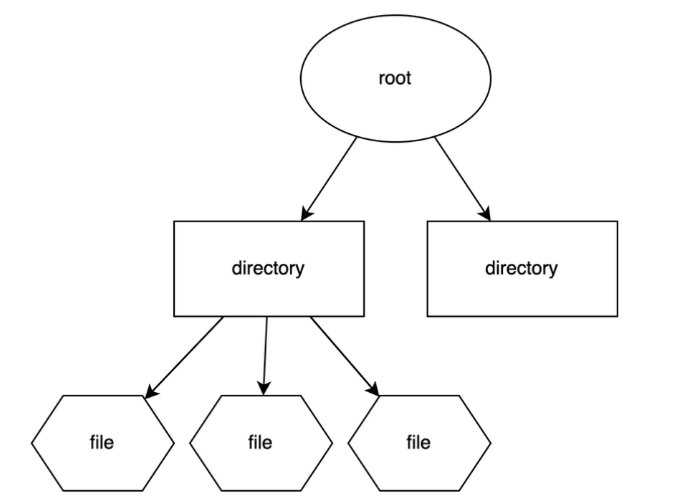
\includegraphics[width=300pt]{./graphics/HFS.png}
    \caption{HFS voorbeeld \autocite{Codecadamy2022}}
    \label{fig:HFS}
\end{figure}

zFS is iets minder bekend en kan gebruikt worden in plaats van of als toevoeging op het traditionele HFS. Dit heeft vooral zijn waarde door zijn sterke performantie in bestanden die vaak worden gebruikt. Het verminderd ook het risico van het verlies in updates omdat het data asynchroon schrijft in plaats van te wachten op een sync interval. Bestanden in dit systeem kunnen aangepast worden door middel van een Application Programming Interface (API) en kunnen zelf in de HFS toegevoegd worden zonder enige problemen. \autocite{IBM2012} \\

\begin{figure}[pt!]
    \centering
    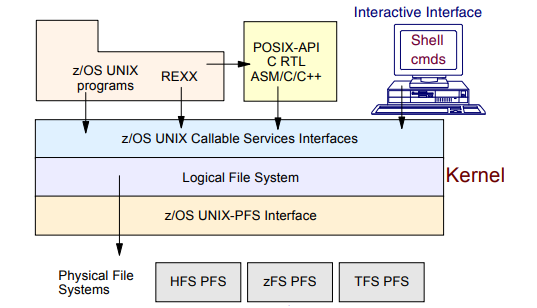
\includegraphics[width=300pt]{./graphics/zFS.png}
    \caption{zFS werking \autocite{IBM2012}}
    \label{fig:zFS}
\end{figure}

In figuur \ref{fig:zFS} worden de bestanden opgehaald vanuit het zFS bestandsysteem door middel van de interactieve interface. Dankzij de API's tussen het logische -en fysieke bestandsysteem worden de juiste bestanden opgehaald en teruggegeven aan de gebruiker. \autocite{IBM2012} \\

Unix bestanden op de mainframe worden bijna op dezelfde manier gebruikt als op een traditioneel unix systeem. Het kan een Java, C++ of Python programma bevatten. Deze programma's kunnen ook bestanden lezen of schrijven in een JSON of YAML formaat. Die kunnen op hun beurt dan gebruikt worden om analyses te doen op bepaalde data. Het hangt allemaal af van de use case om te zien op welke manier deze unix bestanden het best gebruikt worden. \autocite{Precisely2020} \\

Deze omgeving werkt ook met omgevingsvariabelen die invloed hebben op hoe het systeem werkt. Veel van deze variablen worden opgezet bij het inloggen maar de gebruiker kan deze zelf aanpassen. Deze kunnen verwijzen naar de directory waar de gebruiker zich in bevindt, maar zijn ook nodig voor bepaalde packages om hun installatiepad te vinden. \autocite{HenryStocker2017}

\section{Python in z/OS}
Aangezien er een Python interpreter opzetten zal worden, wordt er hier vooral gefocust op Python in z/OS. Dit is één van de meest gebruikte programmeertalen op de dag van vandaag door zijn verschillende doeleinden en begin vriendelijkheid \autocite{Johnson2023}. Ook IBM heeft dit opgemerkt en besloot om dit compatibel te maken met de mainframe. De meest gebruikte doeleinden zijn voor Data analyse -en visualisatie, machine learning en software development. Voor de laatste speelt de flexibiliteit en de kracht van de programmeertaal een grote rol omdat er zowel heel simpele als zeer complexe applicaties geschreven kunnen worden. In software development worden vaak API's ontwikkeld met verschillende packages. \autocite{Kosourova2022} \\

\subsection{Python in USS}
Naast programmeren, heeft dit ook de mogelijkheid om Python commando's uit te voeren in de terminal van USS. Met het python commando kan er bijvoorbeeld een virtuele omgeving aangemaakt worden. Dit is een directory met een bepaalde bestandsstructuur en bevat een bin subdirectory die verwijst naar de Python interpreter en verschillende packages die geïnstalleerd zijn in deze omgeving.  \autocite{UniPrinceton2022} \\
Het is gebouwd op een bestaande Python installatie en gebruikt tools zoals pip om packages te installeren \autocite{PSF2024}. \\

Een Python virtuele omgeving zorgt voor een stabiele en herproduceerbare omgeving waar de gebruiker in volledige controle is over welke packages geïnstalleerd zijn. Hierdoor heeft de gebruiker geen problemen met administratierechten die voorkomen als er niet in deze omgeving gewerkt wordt. Er is geen limiet op het aantal virtuele omgevingen dat een gebruiker kan opstellen en deze zijn gemaakt om eenvoudig te activeren en deactiveren. \autocite{UniPrinceton2022} \\

Bij het aanmaken zijn er verschillende opties mogelijk. De meest belangrijke voor dit onderzoek is de \textit{--system-site-packages} optie. Dit laat de gemaakte virtuele omgeving toe om packages te gebruiken die al geïnstalleerd zijn op het systeem. \autocite{PSF2024}.

Het aanmaken van een Python virtuele omgeving met de packages van het systeem zou als volgt gebeuren:
\begin{lstlisting}
    $ python -m venv /Path/To/venv --system-site-packages
    
\end{lstlisting}

In de meegegeven directory worden subdirectories aangemaakt die nodig zijn om de virtuele omgeving te onderhouden. Om het te activeren, moet het \textit{activate} script in de \textit{bin} subdirectory uitgevoerd worden. \autocite{PSF2024} \\
Afhankelijk van het systeem, wordt een verschillend \textit{activate} script gebruikt. In bash noemt dit \textquote{activate} en wordt uitgevoerd als volgt:
\begin{lstlisting}
    $ source ./bin/activate
    
\end{lstlisting}

Om deze omgeving af te sluiten, wordt volgend commando ingegeven:
\begin{lstlisting}
    $ deactivate
    
\end{lstlisting}

Voor het activeren moet er specifiek verwezen worden naar het \textit{activate} script in de bin subdirectory. Het deactiveren kan in eender welke directory.

\subsection{Packages in Python}
In Python wordt er vaak gebruik gemaakt van externe packages en modules die gebruikt kunnen worden door programmeurs tijdens het schrijven van een applicatie. \\
Een module is een python bestand wat bestaat uit definities en statements. Dit kan bestaan uit variabelen en functies die gerelateerd zijn. Via het \textquote{import} statement, kunnen de functies in een module gebruikt worden in een extern Python applicatie \autocite{Singh2024}. Dit zorgt ervoor dat programmeurs niet zelf de code moeten schrijven waardoor ze veel tijd kunnen winnen. Dit zorgt er ook voor dat repetitieve code niet elke keer opnieuw geschreven moet worden.\\

Een packages is een directory waar verschillende modules in opgeslagen worden en bevatten in sommige gevallen subdirectories. Omdat alles in een directory zit, zijn de modules met elkaar verbonden via de naam van de package. Dit bevat een \textquote{init.py} bestand wat het duidelijk maakt voor Python dat dit een package is. Dit bestand kan leeg zijn of code bevat die uitgevoerd wordt als de package geïnitialiseerd wordt. \autocite{Udacity2021} \\

Een voorbeeld van een package is FastAPI: dit kan gebruikt worden om API's te ontwikkelen. Tijdens het ontwikkelen, wordt er automatisch een interactieve documentatie opgesteld zodat de gebruiker dit niet hoeft te doen. Dit maakt gebruik van een andere package genaamd \textquote{pydantic} en dit zorgt ervoor dat de declaraties van datatypes hetzelfde blijft als in Python. Een andere package genaamd \textquote{starlette} zorgt voor sterke performantie, startup en shutdown events en support voor achtergrond taken tijdens het uitvoeren. \autocite{FastAPI} \\

Om een API uit te voeren, kan er gebruik worden gemaakt van de \textquote{Uvicorn} package. Dit is een web server wat inkomende verzoeken van gebruikers ontvangt. Dit werkt samen met FastAPI om de inkomende verzoeken correct te verwerken. Dit zorgt ervoor dat Uvicorn focust op de netwerk connectie en inkomende verzoeken, en FastAPI op het verwerken van deze verzoeken. \autocite{Sentry2024}

\subsection{Python AI toolkit for z/OS}
Om gebruik te maken van deze packages met modules, moeten deze geïnstalleerd zijn op het systeem en dit kan een probleem zijn in USS. Door de beveiliging op de mainframe is het niet simpel om packages direct te installeren in z/OS \autocite{IBM2021} en hierdoor heeft IBM een Python AI toolkit for z/OS opgezet. \\

In de aankondiging door Evan \textcite{Rivera2023} werd deze toolkit beschreven als een bekende en flexibele ervaring voor developers tijdens het ontwerpen van AI oplossingen. Het biedt open source software aan en deze kunnen eenvoudig geïnstalleerd worden door de Package Installer for Python (pip). \\

De Python AI toolkit is dus een bibliotheek met verschillende, wereldwijd gebruikte Python packages voor AI en Machine learning workloads bijvoorbeeld NumPy, SciPy, Jupyter, etc. Elk van deze packages is volledig onderzocht geweest voor potentiële problemen in het systeem waardoor alles in deze toolkit voldoet aan de beveiligingsvoorwaarden zoals andere z/OS producten. \autocite{Bostian2023}

\subsection{Z Open Automation Utilities}
Python alleen op de mainframe is niet voldoende. Vaak willen developers datasets in z/OS kunnen lezen of schrijven en Python biedt hier geen functies voor aan. IBM is dan opgekomen met de Z Open Automation Utilities (ZOAU). Dit bevat functies om acties uit te voeren op datasets in z/OS of op het systeem zelf. Dit is ontworpen door IBM om het zo natuurlijk mogelijk te laten aanvoelen voor developers die weinig kennis hebben over z/OS. Zo zijn de functies zeer gelijkaardig als hun tegenliggende Unix commando's. Een commando om een lijst van datasets weer te geven bijvoorbeeld is \textit{dls}. Dit is geïnspireerd op het \textit{ls} Unix commando om de inhoud te zien van een bepaalde directory. ZOAU bevat ook een \textit{zopen} statement om datasets te openen voor te lezen of schrijven. In Python is dit het \textit{open} statement. \autocite{IBM2023a}

\section{IBM Developer for z/OS}
\label{sec:IBM Developer for z/OS (IDz)}
\subsection{IDz}
De omgeving waarin er gewerkt zal worden is IBM Developer for z/OS (IDz) versie 16.0.2. Dit programma is volgens de definitie van \textcite{Spohn2023} een toolset voor het ontwikkelen en opzetten van hybride cloud applicaties op z/OS. \\
Het is een Eclipse based programma met de mogelijkheid om een connectie te maken met verschillende omgevingen op de mainframe bijvoorbeeld de USS of z/OS omgeving. Dit biedt de mogelijkheid om alle bestanden te zien, te openen en aan te passen. Omdat de data nogsteeds op de mainframe staat, kunnen wijzigingen direct gezien worden in andere programma's. Als een gebruiker bijvoorbeeld een bestand wijzigt via IDz, kunnen deze wijzigingen direct te zien zijn in ISPF. \\
Dit programma is vooral ontwikkelt om een gekende werkomgeving te bieden om in te programmeren aangezien niet iedereen bekend is met ISPF. \\

Zoals vermeld zal er gebruik worden gemaakt van IDz versie 16.0.2 . In het overzicht van \textcite{IBM2024}, ondersteund deze versie syntax veranderingen voor COBOL 6.4, PL/1 6.1 en REXX. Er is ook een ZUnit update wat vooral het gebruik van deze tool makkelijker maakt. \\

ZUnit staat voor z/OS Automated Unit Testing en is een framework dat gebruikt wordt in IDz om COBOL en PL/1 programma's te testen. Hiervoor maakt het gebruik van verschillende \textquote{samples} die door IBM ontworpen zijn (bv. Enterprise COBOL CALL02.cbl sample test case). Het gebruik van deze tool maakt het makkelijker voor developers om hun code (geschreven in COBOL of Pl/1) te testen op de mainframe. Dit maakt het schrijven van code in IDz veel efficiënter. \autocite{IBM2024a} \\

Het is ook mogelijk om bestanden van de lokale machine te kopiëren naar de mainframe in de USS omgeving. Belangrijk hierbij is de manier waarop het bestand wordt gekopieerd. In IDz noemt dit \textquote{File Transfer Mode} en heeft 2 opties: 
\begin{itemize}
    \item Text
    \item Binary
\end{itemize}
Afhankelijk van het bestand wordt text of binary gekozen en het wordt ingesteld op basis van de extensie van het bestand.

\subsection{Eclipse IDE}
IDz is gebaseerd op de Eclipse Integrated Development Environment (IDE) wat ontwikkeld is door de Eclipse Foundation in 2001. Het is begonnen sinds IBM 3 miljoen lijnen code van hun Java tools heeft gedoneerd om een open source IDE te creëren. Het is dus Java gebaseerd maar kan ook gebruikt worden voor andere programeertalen zoals Python door de verschillende plug-ins die beschikbaar zijn gemaakt door de community achter Eclipse. \autocite{Hanna2021} \\

Plug-ins zijn toevoegingen aan de gebruikte software die het mogelijk maken om applicaties, computer programma's en web browsers aan te passen. Dit zijn ook add ons die extra functionaliteiten kunnen bieden aan het gebruikte programma. \autocite{George2021} 

\subsection{Pydev}
Pydev in een voorbeeld van een plug-in die opgezet kan worden in Eclipse om een Python IDE te gebruiken.  Dit biedt functies zoals code completion, code analysis, debugging, code coverage en nog meer. De meest recente versie is 12.0.0 wat werd uitgebracht op 1 februari 2024. Dit bevatte updates voor de debugger en code analyse. Dit is enkel beschikbaar voor Python 3.8 en hoger waardoor een oudere versie van Pydev nodig is moest een gebruiker een Python versie lager gebruiken. Het is volledig open source en hangt af van externe sponsors om verder ontwikkeld te worden. \autocite{Pydev2024}

\subsection{Wizards}
Een programma zoals IDz heeft veel mogelijkheden om instellingen aan te passen door middel van wizards. Dit is een serie van pagina's dat de gebruiker begeleidt om een complexe taak uit te voeren. Elke pagina vraagt wat informatie en als de gebruiker op 'finish' klikt wordt de taak uitgevoerd. Er is ook altijd een mogelijkheid om het proces stop te zetten. \autocite{Eclipse2006}

\section{IBM Z in een bankomgeving}
Dit onderzoek wordt uitgevoerd in een bankomgeving dus is het interessant om na te gaan welke voordelen een mainframe te bieden heeft in deze omgeving. \\ 

In een aankondiging van \textcite{IBM2022} over hun nieuw systeem de IBM z16, werd er gezegd dat 70\% van wereldwijde transacties door een mainframe verwerkt worden. \\

Volgens \textcite{Turner2022} gebruiken de meeste banken een IBM mainframe omdat ze de rekenkracht kunnen bieden die banken nodig hebben om efficiënt te kunnen werken. Kenmerken zoals robuustheid, betrouwbaarheid en snelle verwerkingskracht spelen ook een grote rol aangezien het van groot belang is dat het systeem bijna altijd actief moet zijn. De mainframe toont hier zijn sterkte door de 8 nines toe te passen. Dit betekent dat een mainframe 99,999999\% van de tijd beschikbaar moet zijn per jaar. \autocite{IBMa} \\

Dit is niet de enige reden waarom het gebruikt wordt door 92 van de top 100 banken ter wereld \autocite{Tozzi2022}. Beveiliging speelt ook een grote rol. Een studie van \textcite{MorningConsult2022} toont aan dat krediet kaart fraude het meest voorkomende type fraude is onder klanten in 7 verschillende landen waaronder Duitsland, de Verenigde Staten en China. de IBM zSystems heeft al een goede transactie beveiliging zonder teveel vertraging maar de z16 brengt hier nog een AI model bij. Hierdoor kunnen banken transacties controleren op een veel grotere schaal: 300 miljard door AI beveiligde transacties per dag met maar 1 milliseconde vertraging. Andere zaken zoals belastingsfraude kunnen ook vermeden worden hiermee. \autocite{IBM2022} \\

IBM doet dit door middel van een nieuwe Telum Processor. Het is ontworpen om deep learning algoritmes naar workloads te brengen voor bedrijven om in real-time fraude te detecteren en te verwerpen. Dit is de eerste processor van IBM dat gebruik maakt van AI terwijl de transactie wordt uitgevoerd. Naast het detecteren van fraude is deze chip nog nuttig voor loan processing, het tegengaan van witwassen van geld en risico analyse. \autocite{IBM2021a} \\

\subsection{Batch \& online jobs}
Batch processen is ook een belangrijk voordeel dat een mainframe te bieden heeft. Dit zijn jobs die uitgevoerd kunnen worden met weinig tot geen interactie van een gebruiker \autocite{IBM}. Dit is vooral nuttig voor taken die op vaste momenten uitgevoerd moeten worden.

In figuur \ref{fig:batch} is een duidelijk voorbeel over hoe een batch job te werk gaat:

\begin{itemize}
    \item[1] De batch job wordt opgestart door de mainframe
    \item[2] De job genereert statistieken van het bedrijf
    \item[3] Er wordt een backup gemaakt van de kritische bestanden en de database voor en na de job
    \item[4] De statistieken worden verstuurd naar een specifieke plaats zodat het geanalyseerd kan worden
    \item[5] Fouten in de statistieken worden in een andere locatie geplaatst
    \item[6] Informatie van klanten hun bankrekening wordt gemaakt en verstuurd.
    \item[7] Een verslag van de verwerkingstijd wordt verstuurd naar de partners van de bank
    \item[8] De partner ontvangt het verslag
    \item[9] Het systeem monitort de uitkomst van de batch job
    \item[10] Jobs en transacties updaten de database zodat de progressie wordt opgeslagen
\end{itemize}
\\ \\
\begin{figure}[p!]
    \centering
    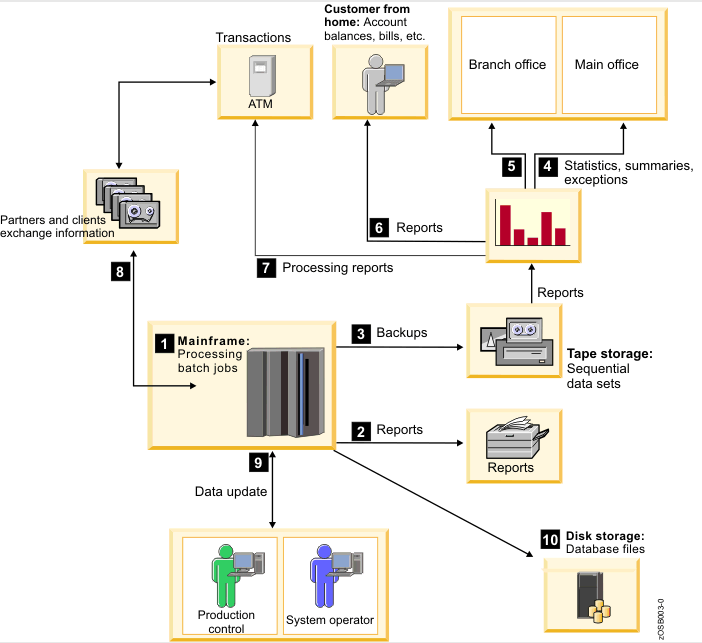
\includegraphics[width=400pt]{./graphics/BatchJobVB.png}
    \caption{Batch Job \autocite{IBMb}}
    \label{fig:batch}
\end{figure}

\begin{figure}[ph!]
    \centering
    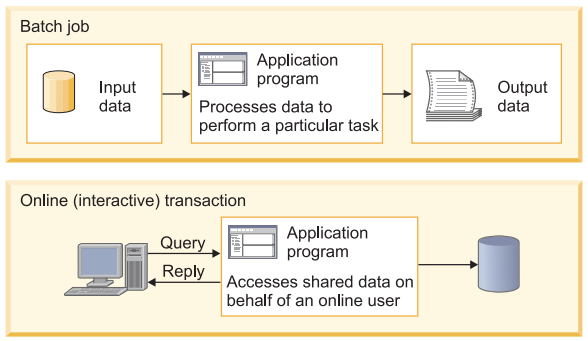
\includegraphics[width=400pt]{./graphics/BatchVSOnline.png}
    \caption{Grafisch verschil tussen batch en OLTP \autocite{IBMb}}
    \label{fig:online}
\end{figure}


Batch jobs zijn niet de enige vorm van jobs die uitgevoerd worden op een mainframe. Online transaction processing of OLTP is zeer belangrijk in een bank. In tegenstelling met batch processing, heeft dit een eindgebruiker nodig die de job opstart. Het heeft ook geen vast moment waarop de job uitgevoerd wordt en kan dus op elk moment van de dag gebeuren. Meestal duren deze transacties niet lang maar de systemen die verantwoordelijk zijn om deze jobs uit te voeren moeten veel verschillende gebruikers op hetzelfde moment ondersteunen zonder enige vertraging. \autocite{IBMb} \\

Een grafische voorstelling van de verschillen tussen een batch job en een online transaction job is te zien in figuur \ref{fig:online}. Een batch job heeft input die verwerkt wordt door een programma op een bepaald, vast moment. De uitkomst wordt dan geschreven in een bestand om analyses op uit te voeren. \\
Een online transactie daarentegen wacht op een query van een gebruiker om te starten. Data wordt dan opgehaald uit het systeem en teruggegeven aan de gebruiker. \autocite{IBMb}


\subsection{Uitvoeren van batch jobs}
Batch jobs worden uitgevoerd door middel van Job Control Language (JCL). Dit zijn aparte programma's die de middelen definiëren die een batch job nodig heeft bijvoorbeeld een input -of output bestand. Een JCL programma bestaat uit 3 statements: 
\begin{itemize}
    \item JOB - Hier wordt de naam van het programma bepaald (jobname). Er kunnen parameters toegevoegd worden die gelden voor de hele job.
    \item EXEC - Dit bepaald het programma dat uitgevoerd moet worden. Een JCL kan meerdere EXEC statements bevatten waarbij elke statement een \textit{job step} wordt genoemd
    \item DD - Dit bepaald de input en/of output bestanden die de batch job nodig heeft.
\end{itemize}
Hoewel dit niet veel functies zijn, bestaan er veel verschillende parameters die meegegeven kunnen worden en die de werking  van het programma zullen beïnvloeden. Dit is wat JCL moeilijk maakt om te schrijven. Dit kan zowel in TSO als in ISPF uitgevoerd worden. \autocite{IBM} \\

In DNB wordt de JCL opgesplitst in 2 programma's:

\begin{itemize}
    \item[1] Job card - Bevat de JOB statement
    \item[2] Procedure - Bevat de EXEC en DD statements
\end{itemize}
Voor het uitvoeren wordt er enkel verwezen naar de Job card en die roept op zijn beurt de procedure op. \\

\newpage
\section{Samenvatting}
Omdat het hoofdbesturingssysteem z/OS van een mainframe niet gekend is door velen en gebruik maakt van verschillende programmeertalen en manieren van data opslaan, heeft IBM ervoor gezorgd dat er een Unix systeem aanwezig is genaamd de USS. Hierdoor kunnen gebruikers die niet bekend zijn met z/OS toch nog gebruik maken van dit systeem. Dit biedt dankzij IBM verschillende tools om packages te installeren en om interactie te hebben met datasets via de Python AI toolkit for z/OS en de Z Open Automation Utilities (ZOAU). Beide zijn beschikbaar voor Python en Java. \\

Via IDz kunnen gebruikers bestanden in de USS openen en aanpassen. Via een externe SSH connectie kunnen deze getest worden. IDz is gebaseerd op Java waardoor er een Java interpreter aanwezig is. Dit is niet het geval voor Python en heeft als gevolg dat er geen Python interpreter aanwezig is. In IDz kan er wel gebruik worden gemaakt van verschillende plug-ins die dit mogelijk kunnen maken. \\

Hoewel de USS omgmeving het eenvoudiger maakt om applicaties te schrijven, is het (voorlopig) niet de bedoeling dat de applicaties die in COBOL of PL/1 geschreven zijn te vervangen worden. Deze programmeertalen zijn zeer belangrijk voor batch en online jobs uit te voeren op  de mainframe en zijn kritisch voor een bedrijf zoals een bank om hun infrastructuur staande te houden en de juiste services te kunnen bieden aan de klanten. \\

De plug-in Pydev speelt een belangrijke rol aangezien dit geimplementeerd wordt in deze bachelorproef. \\

Tenslotte werden Batch en OLTP jobs besproken om zo de hoofdfunctie van een mainframe in een bankomgeving duidelijk te maken.\\

\newpage
\section{Conclusie}
Deze literatuurstudie heeft een overzicht gegeven van IBM hun mainframes om duidelijkheid te scheppen over de omgeving waarin er gewerkt wordt. Dit ging over het hoofdbesturingssysteem z/OS en zijn verschillende onderdelen zoals TSO, ISPF, datasets en programmeertalen. Hoe er gemoderniseerd wordt door IBM door middel van de USS omgeving speelt ook een grote rol. Verschillende tools die gebruikt worden in deze modernisatie zoals IDz, de Python AI toolkit en ZOAU zijn zeer belangrijk om het gebruik van Python en Java zo efficiënt mogelijk te laten gebeuren. \\

Door deze analyse kan er geconcludeerd worden dat Pydev een goede functie kan zijn in IDz aangezien er geen Python interpreter aanwezig is in dit programma. Om het schrijven van Python applicaties nog efficiënter te maken, is dit zeer belangrijk. Aangezien IDz Eclipse based is, zou het geen complexe opgave moeten zijn om dit te implementeren. IDz heeft ook de mogelijkheid om een connectie te maken met de USS omgeving dus is er mogelijks een manier om via IDz Python applicaties uit te voeren op de mainframe. \\

Python en Java zullen meer gebruikt worden door bedrijven omdat ze vrezen voor een sterk werknemerstekort in de toekomst. Hoewel dit onderzoek het eenvoudiger maakt om Python applicaties te schrijven, is het interessant om te onderzoeken of batch en OLTP jobs geschreven in COBOL en PL/1, volledig vervangen kunnen worden door applicaties in de USS omgeving geschreven in Python en Java. \\

%Deze literatuurstudie heeft mijn inzicht in de complexe omgeving van een IBM mainframe sterk doen groeien en mij aangemoedigd om verdere kennis op te doen in het gebied van USS en hoe dit samen met het traditionele z/OS systeem een sterke combinatie kan vormen.